


\tikzset{every picture/.style={line width=0.75pt}} %set default line width to 0.75pt        

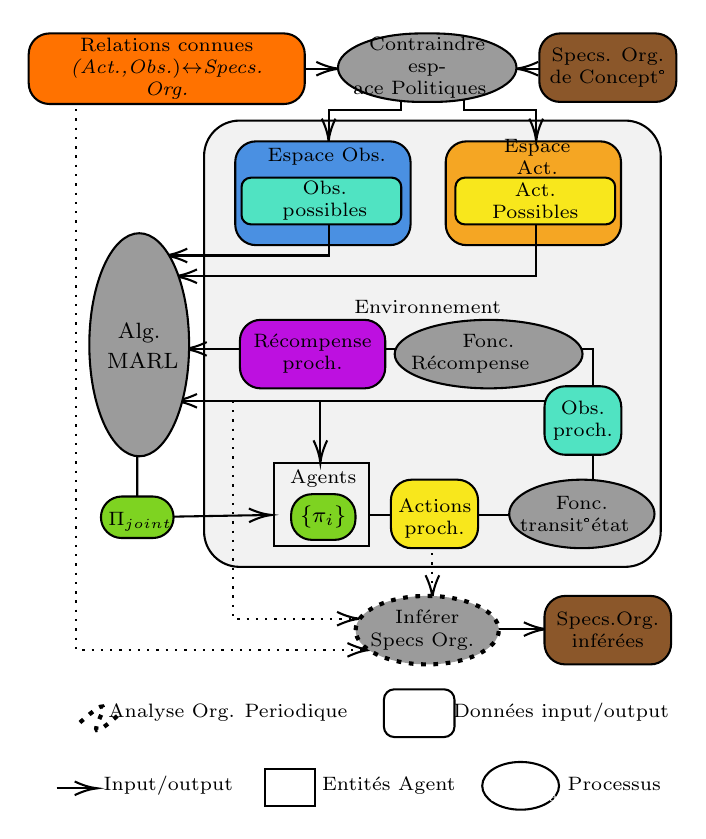
\begin{tikzpicture}[x=0.75pt,y=0.75pt,yscale=-1,xscale=1]
%uncomment if require: \path (0,1886); %set diagram left start at 0, and has height of 1886

%Shape: Rectangle [id:dp9267560871618745] 
\draw  [fill={rgb, 255:red, 242; green, 242; blue, 242 }  ,fill opacity=1 ] (111,1267) .. controls (111,1257.61) and (118.61,1250) .. (128,1250) -- (314,1250) .. controls (323.39,1250) and (331,1257.61) .. (331,1267) -- (331,1448) .. controls (331,1457.39) and (323.39,1465) .. (314,1465) -- (128,1465) .. controls (118.61,1465) and (111,1457.39) .. (111,1448) -- cycle ;
%Straight Lines [id:da07003214167112137] 
\draw    (141.56,1440.03) -- (78.8,1441.11) -- (78.8,1396.11) ;
\draw [shift={(143.56,1440)}, rotate = 179.02] [color={rgb, 255:red, 0; green, 0; blue, 0 }  ][line width=0.75]    (10.93,-3.29) .. controls (6.95,-1.4) and (3.31,-0.3) .. (0,0) .. controls (3.31,0.3) and (6.95,1.4) .. (10.93,3.29)   ;
%Straight Lines [id:da4847818020654431] 
\draw    (298.41,1425) -- (298.41,1360) -- (103.33,1360) ;
\draw [shift={(101.33,1360)}, rotate = 360] [color={rgb, 255:red, 0; green, 0; blue, 0 }  ][line width=0.75]    (10.93,-3.29) .. controls (6.95,-1.4) and (3.31,-0.3) .. (0,0) .. controls (3.31,0.3) and (6.95,1.4) .. (10.93,3.29)   ;
%Straight Lines [id:da28724922448979795] 
\draw    (268.26,1440) -- (190.48,1440) ;
\draw [shift={(270.26,1440)}, rotate = 180] [color={rgb, 255:red, 0; green, 0; blue, 0 }  ][line width=0.75]    (10.93,-3.29) .. controls (6.95,-1.4) and (3.31,-0.3) .. (0,0) .. controls (3.31,0.3) and (6.95,1.4) .. (10.93,3.29)   ;
%Straight Lines [id:da8996673616402417] 
\draw    (167.02,1385) -- (167.02,1394.54) -- (167.02,1413) ;
\draw [shift={(167.02,1415)}, rotate = 270] [color={rgb, 255:red, 0; green, 0; blue, 0 }  ][line width=0.75]    (10.93,-3.29) .. controls (6.95,-1.4) and (3.31,-0.3) .. (0,0) .. controls (3.31,0.3) and (6.95,1.4) .. (10.93,3.29)   ;
%Rounded Rect [id:dp5328357404760626] 
\draw  [fill={rgb, 255:red, 245; green, 166; blue, 35 }  ,fill opacity=1 ] (227.41,1270) .. controls (227.41,1264.48) and (231.89,1260) .. (237.41,1260) -- (301.87,1260) .. controls (307.4,1260) and (311.87,1264.48) .. (311.87,1270) -- (311.87,1300) .. controls (311.87,1305.52) and (307.4,1310) .. (301.87,1310) -- (237.41,1310) .. controls (231.89,1310) and (227.41,1305.52) .. (227.41,1300) -- cycle ;
%Rounded Rect [id:dp7896005679285849] 
\draw  [fill={rgb, 255:red, 248; green, 231; blue, 28 }  ,fill opacity=1 ] (232.1,1282) .. controls (232.1,1279.51) and (234.12,1277.5) .. (236.6,1277.5) -- (304.56,1277.5) .. controls (307.04,1277.5) and (309.06,1279.51) .. (309.06,1282) -- (309.06,1295.5) .. controls (309.06,1297.99) and (307.04,1300) .. (304.56,1300) -- (236.6,1300) .. controls (234.12,1300) and (232.1,1297.99) .. (232.1,1295.5) -- cycle ;
%Straight Lines [id:da4705759557894309] 
\draw    (284.33,1385) -- (98.63,1385) ;
\draw [shift={(96.63,1385)}, rotate = 360] [color={rgb, 255:red, 0; green, 0; blue, 0 }  ][line width=0.75]    (10.93,-3.29) .. controls (6.95,-1.4) and (3.31,-0.3) .. (0,0) .. controls (3.31,0.3) and (6.95,1.4) .. (10.93,3.29)   ;
%Straight Lines [id:da9263936725848416] 
\draw  [dash pattern={on 0.84pt off 2.51pt}]  (124.79,1385) -- (124.79,1490) -- (184,1490) ;
\draw [shift={(186,1490)}, rotate = 180] [color={rgb, 255:red, 0; green, 0; blue, 0 }  ][line width=0.75]    (10.93,-3.29) .. controls (6.95,-1.4) and (3.31,-0.3) .. (0,0) .. controls (3.31,0.3) and (6.95,1.4) .. (10.93,3.29)   ;
%Straight Lines [id:da2407936644656632] 
\draw    (165.39,1225) -- (126,1225) -- (174,1225) ;
\draw [shift={(176,1225)}, rotate = 180] [color={rgb, 255:red, 0; green, 0; blue, 0 }  ][line width=0.75]    (10.93,-3.29) .. controls (6.95,-1.4) and (3.31,-0.3) .. (0,0) .. controls (3.31,0.3) and (6.95,1.4) .. (10.93,3.29)   ;
%Straight Lines [id:da4062676097051594] 
\draw  [dash pattern={on 0.84pt off 2.51pt}]  (49.3,1240) -- (49.3,1505) -- (189,1505) ;
\draw [shift={(191,1505)}, rotate = 180] [color={rgb, 255:red, 0; green, 0; blue, 0 }  ][line width=0.75]    (10.93,-3.29) .. controls (6.95,-1.4) and (3.31,-0.3) .. (0,0) .. controls (3.31,0.3) and (6.95,1.4) .. (10.93,3.29)   ;
%Straight Lines [id:da7412240395305021] 
\draw    (286.34,1225) -- (263,1225) ;
\draw [shift={(261,1225)}, rotate = 360] [color={rgb, 255:red, 0; green, 0; blue, 0 }  ][line width=0.75]    (10.93,-3.29) .. controls (6.95,-1.4) and (3.31,-0.3) .. (0,0) .. controls (3.31,0.3) and (6.95,1.4) .. (10.93,3.29)   ;
%Straight Lines [id:da3956669199032705] 
\draw    (252.2,1495) -- (274,1495) ;
\draw [shift={(276,1495)}, rotate = 180] [color={rgb, 255:red, 0; green, 0; blue, 0 }  ][line width=0.75]    (10.93,-3.29) .. controls (6.95,-1.4) and (3.31,-0.3) .. (0,0) .. controls (3.31,0.3) and (6.95,1.4) .. (10.93,3.29)   ;
%Shape: Rectangle [id:dp8747924601061419] 
\draw   (144.5,1415) -- (190.48,1415) -- (190.48,1455) -- (144.5,1455) -- cycle ;
%Straight Lines [id:da657628783436011] 
\draw    (206,1240) -- (206,1245) -- (171,1245) -- (171,1258) ;
\draw [shift={(171,1260)}, rotate = 270] [color={rgb, 255:red, 0; green, 0; blue, 0 }  ][line width=0.75]    (10.93,-3.29) .. controls (6.95,-1.4) and (3.31,-0.3) .. (0,0) .. controls (3.31,0.3) and (6.95,1.4) .. (10.93,3.29)   ;
%Shape: Boxed Line [id:dp6033407365258088] 
\draw    (40,1571.69) -- (57.58,1571.69) ;
\draw [shift={(59.58,1571.69)}, rotate = 180] [color={rgb, 255:red, 0; green, 0; blue, 0 }  ][line width=0.75]    (10.93,-3.29) .. controls (6.95,-1.4) and (3.31,-0.3) .. (0,0) .. controls (3.31,0.3) and (6.95,1.4) .. (10.93,3.29)   ;
%Shape: Rectangle [id:dp18423344056487378] 
\draw   (140.26,1562.23) -- (164.34,1562.23) -- (164.34,1580) -- (140.26,1580) -- cycle ;
%Curve Lines [id:da2083241343671336] 
\draw [line width=1.5]  [dash pattern={on 1.69pt off 2.76pt}]  (51.18,1540) .. controls (79.4,1514.78) and (41.99,1561.13) .. (70.21,1535.92) ;
%Rounded Rect [id:dp7914798040350324] 
\draw  [fill={rgb, 255:red, 74; green, 144; blue, 226 }  ,fill opacity=1 ] (126,1270) .. controls (126,1264.48) and (130.48,1260) .. (136,1260) -- (200.47,1260) .. controls (205.99,1260) and (210.47,1264.48) .. (210.47,1270) -- (210.47,1300) .. controls (210.47,1305.52) and (205.99,1310) .. (200.47,1310) -- (136,1310) .. controls (130.48,1310) and (126,1305.52) .. (126,1300) -- cycle ;
%Rounded Rect [id:dp7969404700250284] 
\draw  [fill={rgb, 255:red, 80; green, 227; blue, 194 }  ,fill opacity=1 ] (129.04,1282) .. controls (129.04,1279.51) and (131.06,1277.5) .. (133.54,1277.5) -- (201.5,1277.5) .. controls (203.99,1277.5) and (206,1279.51) .. (206,1282) -- (206,1295.5) .. controls (206,1297.99) and (203.99,1300) .. (201.5,1300) -- (133.54,1300) .. controls (131.06,1300) and (129.04,1297.99) .. (129.04,1295.5) -- cycle ;
%Straight Lines [id:da6619730814949483] 
\draw    (93.94,1315) -- (171,1315) -- (171,1300) ;
\draw [shift={(91.94,1315)}, rotate = 0] [color={rgb, 255:red, 0; green, 0; blue, 0 }  ][line width=0.75]    (10.93,-3.29) .. controls (6.95,-1.4) and (3.31,-0.3) .. (0,0) .. controls (3.31,0.3) and (6.95,1.4) .. (10.93,3.29)   ;
%Straight Lines [id:da6703295479126026] 
\draw    (271,1300) -- (271,1325) -- (98.63,1325) ;
\draw [shift={(96.63,1325)}, rotate = 360] [color={rgb, 255:red, 0; green, 0; blue, 0 }  ][line width=0.75]    (10.93,-3.29) .. controls (6.95,-1.4) and (3.31,-0.3) .. (0,0) .. controls (3.31,0.3) and (6.95,1.4) .. (10.93,3.29)   ;
%Straight Lines [id:da6066853523409226] 
\draw  [dash pattern={on 0.84pt off 2.51pt}]  (221,1445) -- (221,1478) ;
\draw [shift={(221,1480)}, rotate = 270] [color={rgb, 255:red, 0; green, 0; blue, 0 }  ][line width=0.75]    (10.93,-3.29) .. controls (6.95,-1.4) and (3.31,-0.3) .. (0,0) .. controls (3.31,0.3) and (6.95,1.4) .. (10.93,3.29)   ;
%Shape: Boxed Line [id:dp9014869733124249] 
\draw    (236,1240) -- (236,1245) -- (271,1245) -- (271,1258) ;
\draw [shift={(271,1260)}, rotate = 270] [color={rgb, 255:red, 0; green, 0; blue, 0 }  ][line width=0.75]    (10.93,-3.29) .. controls (6.95,-1.4) and (3.31,-0.3) .. (0,0) .. controls (3.31,0.3) and (6.95,1.4) .. (10.93,3.29)   ;


% Text Node
\draw (308.64,1569.5) node  [font=\small] [align=left] {{\scriptsize Processus}};
% Text Node
\draw    (245,1570.5) .. controls (245,1564.15) and (253.28,1559) .. (263.5,1559) .. controls (273.72,1559) and (282,1564.15) .. (282,1570.5) .. controls (282,1576.85) and (273.72,1582) .. (263.5,1582) .. controls (253.28,1582) and (245,1576.85) .. (245,1570.5) -- cycle  ;
\draw (263.5,1570.5) node  [font=\small] [align=left] {\begin{minipage}[lt]{22.12pt}\setlength\topsep{0pt}
\begin{center}
\textcolor[rgb]{1,1,1}{{\tiny aassssaa}}
\end{center}

\end{minipage}};
% Text Node
\draw (93.72,1570.5) node  [font=\small] [align=left] {{\scriptsize Input/output}};
% Text Node
\draw (283,1535.42) node  [font=\small] [align=left] {{\scriptsize Données input/output}};
% Text Node
\draw    (197.63,1529) .. controls (197.63,1526.24) and (199.87,1524) .. (202.63,1524) -- (226.63,1524) .. controls (229.39,1524) and (231.63,1526.24) .. (231.63,1529) -- (231.63,1542) .. controls (231.63,1544.76) and (229.39,1547) .. (226.63,1547) -- (202.63,1547) .. controls (199.87,1547) and (197.63,1544.76) .. (197.63,1542) -- cycle  ;
\draw (214.63,1535.5) node  [font=\small] [align=left] {\begin{minipage}[lt]{20.08pt}\setlength\topsep{0pt}
\begin{center}
\textcolor[rgb]{1,1,1}{{\tiny assaaaa}}
\end{center}

\end{minipage}};
% Text Node
\draw (122.5,1535.5) node  [font=\small] [align=left] {{\scriptsize Analyse Org. Periodique}};
% Text Node
\draw (200,1570.5) node  [font=\small] [align=left] {{\scriptsize Entités Agent}};
% Text Node
\draw (169.17,1288.75) node  [font=\scriptsize] [align=left] {\begin{minipage}[lt]{49.56pt}\setlength\topsep{0pt}
\begin{center}
Obs. possibles
\end{center}

\end{minipage}};
% Text Node
\draw (170.11,1267.5) node  [font=\scriptsize] [align=left] {\begin{minipage}[lt]{43.61pt}\setlength\topsep{0pt}
\begin{center}
Espace Obs.
\end{center}

\end{minipage}};
% Text Node
\draw  [fill={rgb, 255:red, 139; green, 87; blue, 42 }  ,fill opacity=1 ]  (275,1489) .. controls (275,1483.48) and (279.48,1479) .. (285,1479) -- (326,1479) .. controls (331.52,1479) and (336,1483.48) .. (336,1489) -- (336,1502) .. controls (336,1507.52) and (331.52,1512) .. (326,1512) -- (285,1512) .. controls (279.48,1512) and (275,1507.52) .. (275,1502) -- cycle  ;
\draw (305.5,1495.5) node  [font=\scriptsize] [align=left] {\begin{minipage}[lt]{38.44pt}\setlength\topsep{0pt}
\begin{center}
Specs.Org.\\inférées
\end{center}

\end{minipage}};
% Text Node
\draw  [color={rgb, 255:red, 0; green, 0; blue, 0 }  ,draw opacity=1 ][fill={rgb, 255:red, 155; green, 155; blue, 155 }  ,fill opacity=1 ][dash pattern={on 1.69pt off 2.76pt}][line width=1.5]   (184,1495.5) .. controls (184,1486.39) and (199.45,1479) .. (218.5,1479) .. controls (237.55,1479) and (253,1486.39) .. (253,1495.5) .. controls (253,1504.61) and (237.55,1512) .. (218.5,1512) .. controls (199.45,1512) and (184,1504.61) .. (184,1495.5) -- cycle  ;
\draw (218.5,1495.5) node  [font=\scriptsize] [align=left] {\begin{minipage}[lt]{44.39pt}\setlength\topsep{0pt}
\begin{center}
Inférer\\Specs Org. \ \ 
\end{center}

\end{minipage}};
% Text Node
\draw  [fill={rgb, 255:red, 248; green, 231; blue, 28 }  ,fill opacity=1 ]  (201,1433) .. controls (201,1427.48) and (205.48,1423) .. (211,1423) -- (233,1423) .. controls (238.52,1423) and (243,1427.48) .. (243,1433) -- (243,1446) .. controls (243,1451.52) and (238.52,1456) .. (233,1456) -- (211,1456) .. controls (205.48,1456) and (201,1451.52) .. (201,1446) -- cycle  ;
\draw (222,1439.5) node  [font=\scriptsize] [align=left] {\begin{minipage}[lt]{26.14pt}\setlength\topsep{0pt}
\begin{center}
Actions\\proch.
\end{center}

\end{minipage}};
% Text Node
\draw  [fill={rgb, 255:red, 126; green, 211; blue, 33 }  ,fill opacity=1 ]  (152.93,1440) .. controls (152.93,1434.48) and (157.41,1430) .. (162.93,1430) -- (173.93,1430) .. controls (179.45,1430) and (183.93,1434.48) .. (183.93,1440) -- (183.93,1442) .. controls (183.93,1447.52) and (179.45,1452) .. (173.93,1452) -- (162.93,1452) .. controls (157.41,1452) and (152.93,1447.52) .. (152.93,1442) -- cycle  ;
\draw (168.43,1441) node  [font=\footnotesize] [align=left] {\begin{minipage}[lt]{18.45pt}\setlength\topsep{0pt}
\begin{center}
$\displaystyle \{\pi _{i}\}$
\end{center}

\end{minipage}};
% Text Node
\draw (168.43,1422.5) node  [font=\scriptsize] [align=left] {\begin{minipage}[lt]{24.96pt}\setlength\topsep{0pt}
\begin{center}
Agents
\end{center}

\end{minipage}};
% Text Node
\draw  [fill={rgb, 255:red, 80; green, 227; blue, 194 }  ,fill opacity=1 ]  (275,1388) .. controls (275,1382.48) and (279.48,1378) .. (285,1378) -- (302,1378) .. controls (307.52,1378) and (312,1382.48) .. (312,1388) -- (312,1401) .. controls (312,1406.52) and (307.52,1411) .. (302,1411) -- (285,1411) .. controls (279.48,1411) and (275,1406.52) .. (275,1401) -- cycle  ;
\draw (293.5,1394.5) node  [font=\scriptsize] [align=left] {\begin{minipage}[lt]{22.57pt}\setlength\topsep{0pt}
\begin{center}
Obs.\\proch.
\end{center}

\end{minipage}};
% Text Node
\draw  [fill={rgb, 255:red, 155; green, 155; blue, 155 }  ,fill opacity=1 ]  (175.5,1224.5) .. controls (175.5,1215.39) and (193.41,1208) .. (215.5,1208) -- (221.5,1208) .. controls (243.59,1208) and (261.5,1215.39) .. (261.5,1224.5) .. controls (261.5,1233.61) and (243.59,1241) .. (221.5,1241) -- (215.5,1241) .. controls (193.41,1241) and (175.5,1233.61) .. (175.5,1224.5) -- cycle  ;
\draw (218.5,1224.5) node  [font=\scriptsize] [align=left] {\begin{minipage}[lt]{55.91pt}\setlength\topsep{0pt}
\begin{center}
Contraindre esp-\\ace Politiques \ \ \ 
\end{center}

\end{minipage}};
% Text Node
\draw  [fill={rgb, 255:red, 255; green, 114; blue, 0 }  ,fill opacity=1 ]  (26.5,1218) .. controls (26.5,1212.48) and (30.98,1208) .. (36.5,1208) -- (149.5,1208) .. controls (155.02,1208) and (159.5,1212.48) .. (159.5,1218) -- (159.5,1232) .. controls (159.5,1237.52) and (155.02,1242) .. (149.5,1242) -- (36.5,1242) .. controls (30.98,1242) and (26.5,1237.52) .. (26.5,1232) -- cycle  ;
\draw (93,1225) node  [font=\scriptsize] [align=left] {\begin{minipage}[lt]{87.59pt}\setlength\topsep{0pt}
\begin{center}
Relations connues\\\textit{(Act.,Obs.})$\displaystyle \leftrightarrow $\textit{Specs. Org.}
\end{center}

\end{minipage}};
% Text Node
\draw  [fill={rgb, 255:red, 189; green, 16; blue, 224 }  ,fill opacity=1 ]  (128.27,1356) .. controls (128.27,1350.48) and (132.74,1346) .. (138.27,1346) -- (188.27,1346) .. controls (193.79,1346) and (198.27,1350.48) .. (198.27,1356) -- (198.27,1369) .. controls (198.27,1374.52) and (193.79,1379) .. (188.27,1379) -- (138.27,1379) .. controls (132.74,1379) and (128.27,1374.52) .. (128.27,1369) -- cycle  ;
\draw (163.27,1362.5) node  [font=\scriptsize] [align=left] {\begin{minipage}[lt]{44.8pt}\setlength\topsep{0pt}
\begin{center}
Récompense\\proch.
\end{center}

\end{minipage}};
% Text Node
\draw  [fill={rgb, 255:red, 155; green, 155; blue, 155 }  ,fill opacity=1 ]  (258,1439.5) .. controls (258,1430.39) and (273.67,1423) .. (293,1423) .. controls (312.33,1423) and (328,1430.39) .. (328,1439.5) .. controls (328,1448.61) and (312.33,1456) .. (293,1456) .. controls (273.67,1456) and (258,1448.61) .. (258,1439.5) -- cycle  ;
\draw (293,1439.5) node  [font=\scriptsize] [align=left] {\begin{minipage}[lt]{44.87pt}\setlength\topsep{0pt}
\begin{center}
Fonc.\\transit°état \ \ \ 
\end{center}

\end{minipage}};
% Text Node
\draw  [fill={rgb, 255:red, 126; green, 211; blue, 33 }  ,fill opacity=1 ]  (61.3,1441.11) .. controls (61.3,1435.58) and (65.78,1431.11) .. (71.3,1431.11) -- (86.3,1431.11) .. controls (91.82,1431.11) and (96.3,1435.58) .. (96.3,1441.11) .. controls (96.3,1446.63) and (91.82,1451.11) .. (86.3,1451.11) -- (71.3,1451.11) .. controls (65.78,1451.11) and (61.3,1446.63) .. (61.3,1441.11) -- cycle  ;
\draw (78.8,1441.11) node  [font=\scriptsize] [align=left] {\begin{minipage}[lt]{20.95pt}\setlength\topsep{0pt}
\begin{center}
$\displaystyle \Pi _{joint}$
\end{center}

\end{minipage}};
% Text Node
\draw  [fill={rgb, 255:red, 155; green, 155; blue, 155 }  ,fill opacity=1 ]  (79.74, 1358) circle [x radius= 24.04, y radius= 53.74]   ;
\draw (79.74,1358) node  [font=\small] [align=left] {\begin{minipage}[lt]{23.12pt}\setlength\topsep{0pt}
\begin{center}
    \phantom{X}\\{\footnotesize Alg.}\\{\footnotesize MARL}\\\phantom{X}
\end{center}

\end{minipage}};
% Text Node
\draw (270.58,1288.75) node  [font=\scriptsize] [align=left] {\begin{minipage}[lt]{47.57pt}\setlength\topsep{0pt}
\begin{center}
Act. Possibles
\end{center}

\end{minipage}};
% Text Node
\draw (271.52,1267.5) node  [font=\scriptsize] [align=left] {\begin{minipage}[lt]{40.43pt}\setlength\topsep{0pt}
\begin{center}
Espace Act.
\end{center}

\end{minipage}};
% Text Node
\draw (217.23,1337.5) node  [font=\scriptsize] [align=left] {\begin{minipage}[lt]{50.75pt}\setlength\topsep{0pt}
\begin{center}
Environnement
\end{center}

\end{minipage}};
% Text Node
\draw  [fill={rgb, 255:red, 155; green, 155; blue, 155 }  ,fill opacity=1 ]  (202.83,1362.5) .. controls (202.83,1353.39) and (223.09,1346) .. (248.08,1346) .. controls (273.07,1346) and (293.33,1353.39) .. (293.33,1362.5) .. controls (293.33,1371.61) and (273.07,1379) .. (248.08,1379) .. controls (223.09,1379) and (202.83,1371.61) .. (202.83,1362.5) -- cycle  ;
\draw (248.08,1362.5) node  [font=\scriptsize,xslant=-0.02] [align=left] {\begin{minipage}[lt]{58.68pt}\setlength\topsep{0pt}
\begin{center}
Fonc.\\Récompense \ \ \ \ \ \ 
\end{center}

\end{minipage}};
% Text Node
\draw  [fill={rgb, 255:red, 139; green, 87; blue, 42 }  ,fill opacity=1 ]  (272.5,1218) .. controls (272.5,1212.48) and (276.98,1208) .. (282.5,1208) -- (328.5,1208) .. controls (334.02,1208) and (338.5,1212.48) .. (338.5,1218) -- (338.5,1231) .. controls (338.5,1236.52) and (334.02,1241) .. (328.5,1241) -- (282.5,1241) .. controls (276.98,1241) and (272.5,1236.52) .. (272.5,1231) -- cycle  ;
\draw (305.5,1224.5) node  [font=\scriptsize] [align=left] {\begin{minipage}[lt]{42.1pt}\setlength\topsep{0pt}
\begin{center}
Specs. Org.\\de Concept°
\end{center}

\end{minipage}};


\end{tikzpicture}